\documentclass[10pt, a4paper, spanish]{article}
\usepackage[paper=a4paper, left=1.5cm, right=1.5cm, bottom=1.5cm, top=3.5cm]{geometry}
\usepackage[utf8]{inputenc}
\usepackage[spanish,es-nodecimaldot]{babel}
\usepackage{caratula}
\usepackage[pdfencoding=auto, colorlinks=true, linkcolor=blue]{hyperref}
\usepackage[boxruled, longend]{algorithm2e}
\usepackage{wrapfig}
% \usepackage{tikz}
\usepackage[rightcaption]{sidecap}
% \usetikzlibrary{babel}
\graphicspath{imagenes/}

% \tikzset{nodeList/.style={every node/.style={draw, circle}}}
% \tikzset{pathList/.style={every node/.style={midway, fill=white}}}


\newcommand{\ord}{\ensuremath{\operatorname{O}}}
\newcommand{\nat}{\ensuremath{\mathbb{N}}}

\begin{document}
% CARATULA
\materia{Sistemas operatornameerativos}
\submateria{Segundo Cuatrimestre de 2017}
\fecha{\today}
\grupo{}
\titulo{Trabajo Práctico 1}

\integrante{Tarrío, Ignacio}{363/15}{itarrio@dc.uba.ar}
\integrante{Szperling, Sebastián Ariel}{763/15}{sszperling@dc.uba.ar}
\integrante{Balbachan, Alexis}{994/12}{alexisbalbachan@gmail.com}

\maketitle

\newpage
\tableofcontents

\newpage
\section{Introducción}

El propósito de este trabajo práctico es experimentar con \texttt{pthreads}, tanto por los beneficios que trae (en particular en terminos en de performance) y los desafíos que presenta (al sincronizar los varios hilos de ejecución y mantener consistencia). En este TP se implementa un ConcurrentHashMap simplificado que alberga strings y contadores de las mismas.

Para completar el trabajo práctico debimos completar una Lista Atómica provista por la cátedra, y así como implementar desde cero el ConcurrentHashMap, utilizando la Lista previamente mencionada.

\section{Lista Atómica}

La lista se encontraba mayormente implementada, salvo por una operación: \texttt{push\_front}. Esta operación es la única que modifica la lista en sí (si ignoramos la modificación de sus elementos), por lo que esta operación es la que hace a la lista ''atómica``.

Nos dimos cuenta que, como modificar un puntero no es una operación atómica, no bastaría con cargar el nuevo valor para la cabeza de la lista, o podríamos perder elementos. Nuestro primer enfoque hacía un exchange atómico con la nueva cabeza, y luego cargaba la cabeza anterior como siguiente elemento. Esta operación no era puramente atómica, y pudimos hayar casos donde se daba una \textit{race condition} y, si bien los elementos eran perdidos permanentemente, si desaparecían durante un corto lapso, durante el cual la cabeza no conocía a los elementos que estaban anteriormente.

La operación que utilizamos en la versión final es un \texttt{atomic\_compare\_exchange\_weak}, un compare-and-swap que garantiza que, al insertar el nuevo elemento, el mismo apunta al último nodo agregado exitosamente. Como el compare-and-swap no necesariamente es exitoso al principio (alguien puede haber cargado un nuevo valor desde la última vez que fue leído), este compare-and-swap está en un loop hasta que el elemento puede ser insertado sin interrupción.

Esto significa que la inserción no necesariamente coincide con el orden en que fueron llamadas, sino que depende de los cambios de contexto/thread.

\section{ConcurrentHashMap}

El ConcurrentHashMap implementado toma ciertas medidas para permitir que ciertas operaciones (pero no todas) puedan ser ejecutadas en paralelo:

\begin{itemize}

	\item Un contador de operaciones, el cual tendrá dos utilidades en la clase: vitar que se ejecute \texttt{addAndInc} cuando se está ejecutando \texttt{maximum} y vice-versa; y saber cuántas de estas operaciones se están ejecutando. Si el valor de este contador es positivo quiere decir que se están ejecutando ese número de \texttt{addAndInc}, y si es negativo se está ejecutando \texttt{maximum}.

	\item Un mutex que proteje dicho contador y evita que dos operaciones conflictivas se inicien accidentalmente al mismo tiempo.

	\item Una variable de condición que genera un broadcast cuando el contador llega a 0, permitiendo que las tareas que no podían ejecutarse lo hagan ahora y evitando el busy waiting.

	\item Una lista de mutexes, uno por cada fila de la tabla del hashmap, para proteger dichas filas y evitar el agregado de elementos duplicados (ya que \texttt{addAndInc} puede ser concurrente con si mismo).

\end{itemize}

Por otro lado, la operación \texttt{member} es \textit{wait-free}, e ignora todos los locks. Como usamos la Lista Atómica, estamos seguros que la ejecución coincide a alguna ejecución secuencial: esto quiere decir, si bien es posible que el método devuelva \texttt{false} luego de que algo fue agregado, no es posible, luego de un resultado \texttt{true}, obtener un resultado \texttt{false} (que podría haber sucedido si la lista no estuviese implementada atómicamente, como en el ejemplo descrito anteriormente).

Entre otras cosas, también consideramos al implementar el HashMap:

\begin{itemize}

	\item Utilizar un mutex en lugar de una variable de condición, pero lo consideramos ineficiente y propenso a condiciones de carrera (mientras que este es el caso de uso exacto de una variable de condición).

	\item Utilizar \texttt{std::atomic\_uint} en lugar de \texttt{unsigned int} para las entradas del HashMap, pero resulto más sencillo usar el tipo primitivo dada la firma del método a cumplir y que un mutex por fila seguría siendo necesario en ciertos contextos.

\end{itemize}

Como nota al margen, nos encontramos con una dificultades relacionadas con como C y C++ manejan la memoria y los constructores por copia/operadores de asignación:

\begin{itemize}

	\item las clases \texttt{std::mutex}, \texttt{std::atomic} y otras primitivas de sincronización de la biblioteca STD de C++ eliminan explicitamente sus constructores y operadores de asignación por copia, eliminando a su vez los del ConcurrentHashMap y la Lista Atómica. Si bien estas clases contienen utilidades para evitar errores (como lock guards), optamos por utilizar los structs provistos en \texttt{pthread.h} (como \texttt{pthread\_mutex\_t}) para simplificar nuestra implementación.

	\item Al asignar un ConcurrentHashMap, C debe copiarlo a su destino. Sin embargo, como nuestra tabla es una lista de punteros a Listas Atómicas, y las mismas no cuentan con constructor por copia, utilizamos \texttt{std::shared\_ptr} en lugar de punteros puros. De esta forma, cuando el HashMap es copiado y luego destruído, la tabla no es destruída, y las listas que fueron reemplazadas sí. Esto viene con la desventaja que la "copia" no es enteramente tal, y si se realiza una copia y se modifica, la tabla original también es modificada. Sin embargo, esto no debería afectar el caso de uso de este TP.

\end{itemize}

\section{Uso de threads}

Para la implementación de las funciones concurrentes tuvimos que tener en cuenta los siguientes detalles:

\begin{itemize}

	\item Para usar \texttt{pthreads}, consideramos conveniente definir structs relacionados a cada función a ser llamada desde los threads auxiliares. Estos structs contienen casi exclusivamente punteros/referencias.

	\item Para la mayoría de los casos, para evitar el cálculo duplicado de resultados utilizamos contadores atómicos. De esta forma, cada thread estaba informado de si había más trabajo para hacer, o si estaba finalizado.

	\item En el caso de \texttt{maximum}, como el mismo utiliza concurrencia interna y debe publicar un único resultado, también utilizamos una variable atómica para el máximo encontrado, con publicación de resultado via compare-and-swap (al igual que la Lista Atómica). Originalmente utilizamos un mutex para este mismo propósito, pero consideramos que un CAS era probablemente más eficiente que un lock.

	\item Originalmente habíamos implementado esto con \texttt{std::thread}, que tiene una implementación más sencilla (se pueden pasar parámetros arbitrarios en lugar de crear un struct). Sin embargo, entendemos que está fuera del scope de este TP, por lo que reimplementamos todo con \texttt{pthreads}.

\end{itemize}

\newpage
\section{Experimentación}

Hicimos unas pruebas del tiempo de ejecución de las dos versiones de

\begin{center}
	\texttt{static pair<string, uint> ConcurrentHashMap::maximum\\(uint p\_archivos, uint p\_maximos, list<string> archs);}
\end{center}

correspondientes a los ejercicios 5 y 6 del trabajo práctico. La versión del ejercicio 5 no utiliza la versión concurrente de \texttt{ConcurrentHashMap::count\_words}, y la versión del ejercicio 6 (llamada \texttt{maximum\_6} para desambiguar) sí.

\begin{center}
	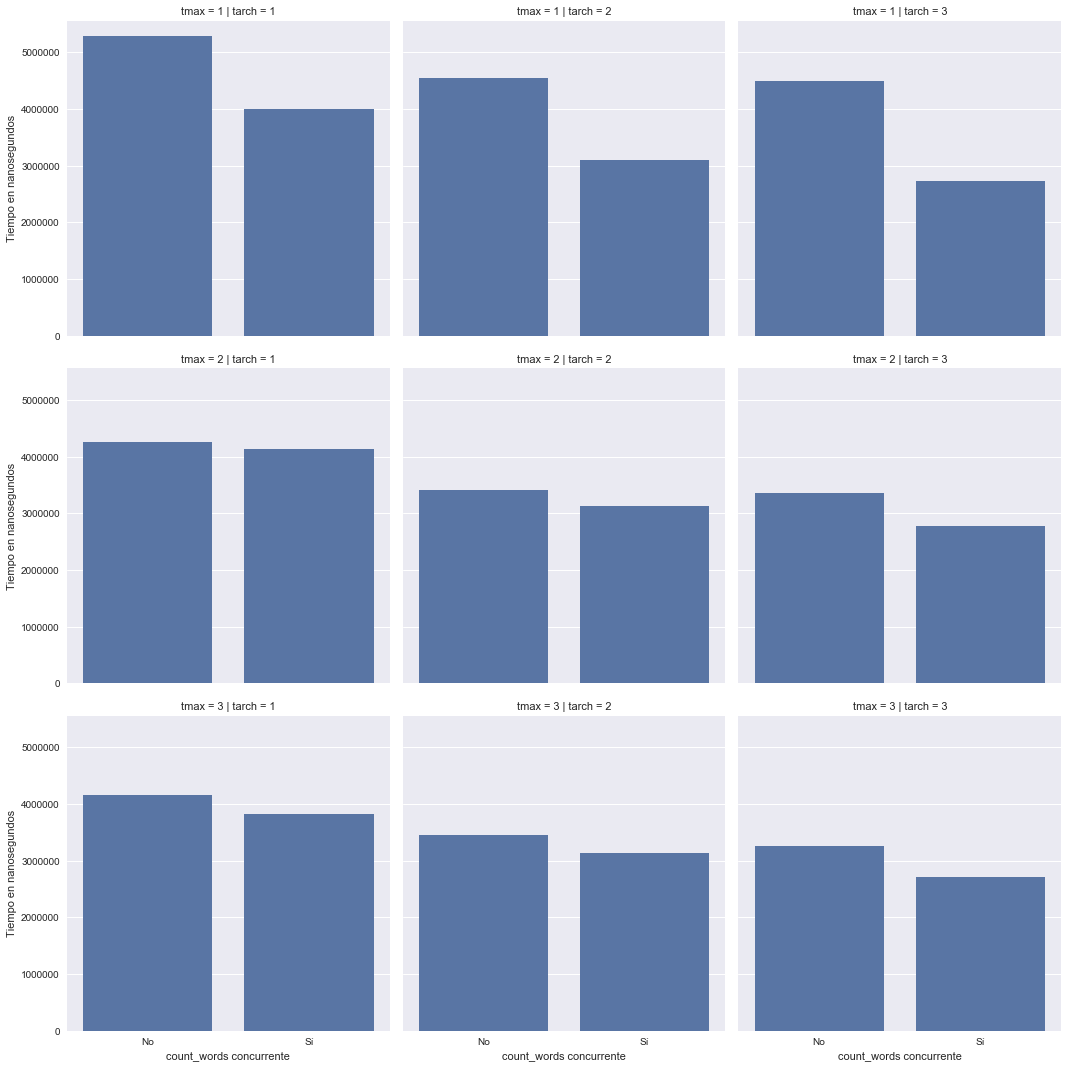
\includegraphics[scale=0.45]{imgs/5-vs-6.png}
\end{center}

En este gráfico se pueden apreciar 2 cosas:

\begin{itemize}

	\item la mejora de performance al utilizar threads es muy notoria, aunque la diferencia al agregar el 2do thread es mayor a la de agregar el 3er thread;

	\item la función que utiliza la versión con concurrencia de \texttt{ConcurrentHashMap::count\_words} puede hacer mejor uso de los threads que tiene disponibles, en particular durante la carga de los archivos, lo que era esperable ya que en la versión no concurrente se generan varios HashMaps y se deben copiar esos resultados a un único HashMap. También suponemos que, dado que todos los HashMaps almacenan sus datos en orden y tienen mutexes por fila de la tabla, es posible que haya muchas esperas durante la copia al HashMap unificado.

\end{itemize}

\newpage
\section{Conclusiones}

Por lo que pudimos observar, el uso de threads puede incrementar enormemente la performance de las aplicaciones más sencillas. Sin embargo, el manejo de threads no es sencillo y debe realizarse con cuidado: por un lado, sin las estructuras de sincronización correctas, es muy facil generar inconsistencias, perder datos, etc.; por el otro, un uso excesivo de estas estructuras también puede tener un impacto pesado en el rendimiento, deshaciendo el beneficio obtenido al paralelizar; por úlitmo, el abuso de los mismos threads puede resultar en trabajo innecesario y perdida de ciclos de procesamiento.

% compilar 2 veces para actualizar las referencias


\end{document}